\documentclass[twocolumn]{IEEEtran} % LaTeX2e
\usepackage{amssymb,amsmath,graphicx,float}

\newcommand\real{\mathbb{R}}

\begin{document}

\title{Model predictive control of a mobile robot using a successive-linearization approach}

\author{\vskip 1em
Felipe K\"{u}hne, Walter F. Lages and Jo\~{a}o Manoel G. da Silva Jr.\\
\vskip 1em
{\small Federal University of Rio Grande do Sul\\
Department of Electrical Engineering\\
Av. Oswaldo Aranha, 103, Porto Alegre, RS, CEP 90035-190, Brazil\\
{\tt \{kuhne,fetter,jmgomes\}@eletro.ufrgs.br}}}

\maketitle


\begin{abstract}
This paper presents an optimal control scheme for trajectory tracking of a wheeled mobile robot (WMR) with nonholonomic constraints. It is well known that a WMR with nonholonomic constraints cannot be feedback stabilized through continuously differentiable, time-invariant control laws. Using model predictive control (MPC), a discontinuous control law is naturally obtained. One of the main advantages of MPC is the ability to handle constraints (due to state or input limitations) in a straightforward way. Quadratic programming (QP) is used to solve a linear MPC by successive linearization of an error model of the WMR. Simulation results are shown.
\end{abstract}
\begin{keywords}
Wheeled mobile robots, model predictive control, trajectory tracking.
\end{keywords}
\thispagestyle{empty}\pagestyle{empty}


\section{Introduction}\label{sec:intro}
The field of mobile robot control has been the focus of great research effort in the past decades. Besides the apparent simplicity of the kinematic model of a wheeled mobile robot (WMR), the existence of nonholonomic (or non-integrable) constraints turns the design of stabilizing control laws for that systems a great challenge, and due to Brocket's conditions \cite{brockett82}, a continuously differentiable, time-invariant stabilizing feedback control law cannot be obtained. Most works in that direction uses discontinuous (non-smooth) and time-variant control laws (see \cite{bloch89,samson91,canudas92,yamamoto94,murray97} and the references therein). Recent works dealing with robust and adaptive control of WMR's can be found in \cite{oya03,dixon04}.

However, in general, for realistic implementations it is difficult to obtain good performance, due to the constraints on input or state that naturally exist. None of the above cited authors have taken those constraints into account. This can be done in a straightforward way using model predictive control (MPC) schemes. For a WMR this is an important advantage, because the position of the robot can be restricted to belong to a secure region of operation (imagine a WMR crossing a corridor, for example). With input limitations, the control actions can be limited to prevent actuators' saturations.

MPC is a control strategy that uses the model of the system being controlled to obtain an optimal control sequence by minimizing an objective function. At each sample interval, the model provides a prediction of process states over a prediction horizon. Based on that, an objective function is optimized with respect to the future open-loop control system inputs. Although prediction and optimization are computed over a future horizon, only the values of the inputs for the current sample interval are used and the same procedure is repeated at the next sample instant. This mechanism is known as {\it moving} or {\it receding horizon} strategy, in reference to the way in which the time window considered in the calculations shifts forward from one time step to the next.

For complex constrained multivariable control problems, MPC has become the accepted standard in the process industries \cite{bemporad02}. It was very well used in such cases, specially where plants being controlled are sufficiently {\em slow} to permit its implementation \cite{mayne98}. However, for systems with fast and/or nonlinear dynamics, like the WMR's, the implementation of such technique remains fundamentally limited in applicability, due to large amount of {\em on-line} computation required \cite{cannon00}. In this paper we overcome this problem by using a successive-linearization approach, where a linear MPC is solved by quadratic programming (QP) problem. With some simulations results, it is shown that even a real-time implementation is possible. Although MPC is not a new control method, works dealing with MPC of WMR's are recent and sparse \cite{ollero91,rico99,essen01}.

The remainder of this paper is organized as follows: in the next section the kinematic model of the WMR is shown. The MPC algorithm is depicted in Section \ref{sec:mpc}. Simulation results in {\sc matlab} are shown in Section \ref{sec:simulations}, where an eight-like trajectory is used as reference. The paper finishes with the conclusions. 


\section{Kinematic model of the WMR}\label{sec:model}
In this section the kinematic model of the WMR is described. A mobile robot made up of a rigid body and non deformable wheels is considered and depicted in Fig. \ref{fig:robot}. It is assumed that the vehicle moves without slipping in an horizontal ground. The kinematics of the WMR is given by:
\begin{equation}\label{eqn:model}
	\left\{
		\begin{aligned}
			\dot x	  &= v\cos\theta \\
			\dot y	  &= v\sin\theta \\
			\dot \theta &= w \\
		\end{aligned}
	\right.
\end{equation}
${\bf x}\triangleq[x~~y~~\theta]^T$ describes the configuration (position and orientation) of the center of mass $C$ with respect to a global inertial frame $\{O,X,Y\}$. ${\bf u}\triangleq[v~~w]^T$ are the manipulated (control) variables, where $v$ and $w$ are the forward and the angular velocity, respectively.
\begin{figure}[t]\begin{center}
    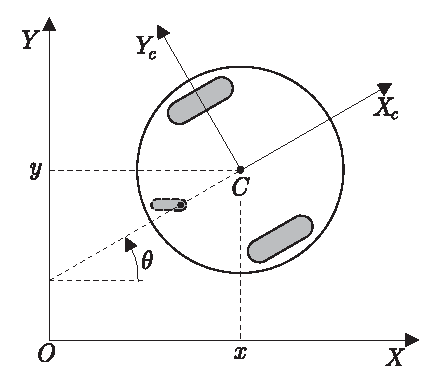
\includegraphics[width=.67\linewidth]{Figures/robot.eps}
    \caption{Kinematic model of the WMR.}
    \label{fig:robot}
\end{center}\end{figure}

Discretizing (\ref{eqn:model}) by the Euler method, i.e.,
\begin{equation*}
	\dot{\bf x} \approx \frac{{\bf x}(k+1)-{\bf x}(k)}{T},
\end{equation*}
where $T$ is the sampling time and $k$ is the sampling step, we have the following nonlinear, discrete-time model:
\begin{equation}\label{eqn:discretemodel}
	\left\{
		\begin{aligned}
			x(k+1)	    &= x(k) + v(k)\cos\theta(k)T \\
			y(k+1)	    &= y(k) + v(k)\sin\theta(k)T \\
			\theta(k+1) &= \theta(k) + w(k)T \\
		\end{aligned}
	\right.
\end{equation} 

\subsection{Derivation of a linear error model}
The kinematic model can be redefined as a new system with relation to deviations from a reference trajectory . This can be done by means of Taylor series, which will provide a linear, time-variant error model that will be used in Section \ref{sec:mpc} for the solution of a linear MPC problem. 

Let consider (\ref{eqn:discretemodel}) equivalent to ${\bf x}(k+1)=f({\bf x}(k),{\bf u}(k))$. Using Taylor series expansion, ignoring the high order terms and evaluating at a reference point $({\bf x}_r(k),{\bf u}_r(k))$, we have the following expression:
\begin{align*}
	f({\bf x}(k),{\bf u}(k)) &\approx f({\bf x}_r(k),{\bf u}_r(k)) + \\ &+ \left.\frac{\partial f}{\partial{\bf x}(k)}\right|_{\begin{smallmatrix}{\bf x}(k)={\bf x}_r(k) \\ {\bf u}(k)={\bf u}_r(k) \end{smallmatrix}}({\bf x}(k)-{\bf x}_r(k)) + \\ &+ \left.\frac{\partial f}{\partial{\bf u}(k)}\right|_{\begin{smallmatrix}{\bf x}(k)={\bf x}_r(k) \\ {\bf u}(k)={\bf u}_r(k) \end{smallmatrix}}({\bf u}(k)-{\bf u}_r(k))
\end{align*}

Noting that ${\bf x}_r(k+1)=f({\bf x}_r(k),{\bf u}_r(k))$, the expression above can be rewritten as:
\begin{equation}\label{eqn:error}
	\tilde{\bf x}(k+1) = {\bf A}(k)\tilde{\bf x}(k)+{\bf B}(k)\tilde{\bf u}(k),
\end{equation}
where, for the kinematic model (\ref{eqn:discretemodel}), we have
\begin{equation*}
	\tilde{\bf x}(k) \triangleq \begin{bmatrix}
		\cos\theta_r(k)  & \sin\theta_r(k) & 0 \\
		-\sin\theta_r(k) & \cos\theta_r(k) & 0 \\
		0		       & 0		     & 1
	\end{bmatrix} 
	\begin{bmatrix}
		x(k)-x_r(k) \\ y(k)-y_r(k) \\ \theta(k)-\theta_r(k)
	\end{bmatrix},
\end{equation*}
$\tilde{\bf u}(k)\triangleq{\bf u}(k)-{\bf u}_r(k)$ and
\begin{align*}
	{\bf A}(k) &= \begin{bmatrix}
		1 & 0 & -v_r(k)\sin\theta_r(k)T \\
		0 & 1 &  v_r(k)\cos\theta_r(k)T \\
		0 & 0 & 1
	\end{bmatrix} \\
	{\bf B}(k) &= \begin{bmatrix}
		\cos\theta_r(k)T & 0 \\
		\sin\theta_r(k)T & 0 \\
		0 			  & T
	\end{bmatrix}
\end{align*}

Indeed, the convergence of ${\bf x}$ to ${\bf x}_r$ is equivalent to the convergence of $\tilde{\bf x}$ to the set ${\cal O}=\{{\bf x}|(\tilde x,\tilde y,\tilde\theta)=(0,0,2\pi n)\},n\in \{0,\pm1,\pm2,\ldots\}$.

Bloch and McClamroch \cite{bloch89} have shown that the nonlinear, nonholonomic system of (\ref{eqn:model}) is fully controllable, i.e., it can be steered from any initial state to any final state in finite time by using finite inputs. It is easy to note that the linearization about a stationary operating point, when the car is motionless, is not controllable. However, this linearization becomes controllable as long as the control inputs ${\bf u}$ are existing \cite{samson91}. This implies that the tracking of a reference trajectory would be possible with linear MPC \cite{essen01}.


\section{The MPC Algorithm}\label{sec:mpc}
As cited in Section \ref{sec:intro}, the essence of a MPC scheme is to optimize, over the control inputs, predictions of process behavior. Such prediction is accomplished using a process model over a finite time interval, called the {\em prediction horizon}. At each sample time, the model predictive controller generates an optimal control sequence by solving a minimization problem. The first element of this sequence is applied to the plant being controlled. The problem is solved again at the next time interval using updated process measurements and a shifted horizon.

In this work, for simplicity we assume that the states of the plant are always available for measure, and that there are no plant/model mismatch (the linearized plant and the linearized model are exactly the same). Also, in order to design the linear controller, it is assumed that the pair $({\bf A}(k),{\bf B}(k))$ is always (at any $k$) stabilizable.

Usually, the optimization problem can be written as:
\begin{equation*}
	\varphi^\star = \arg\min_{\bf\varphi}\left\{\Phi(k)\right\}
\end{equation*}
s. t.
\begin{equation*}\label{eqn:constr}
	{\bf\varphi}_{min} \leq {\bf\varphi} \leq {\bf\varphi}_{max}
\end{equation*}

$\Phi(k)$ is the so called {\em cost function} and usually, for linear systems, takes a quadratic form. ${\bf\varphi}$ is the free variable in the optimization, and ${\bf\varphi}_{min}$ and ${\bf\varphi}_{max}$ are its inferior and superior limits, respectively.

The cost function to be minimized is the following:
\begin{multline}\label{eqn:cost}
	\Phi(k) = \sum_{j=1}^{N}\tilde{\bf x}^T(k+j|k){\bf Q}\tilde{\bf x}(k+j|k) + \\ + \tilde{\bf u}^T(k+j-1|k){\bf R}\tilde{\bf u}(k+j-1|k),
\end{multline}
where $N$ is the prediction horizon and ${\bf Q}$, ${\bf R}$ are weighting matrices, with ${\bf Q}\geq 0$ and ${\bf R}>0$. The free variable is, in this case, the control error $\tilde{\bf u}$. The notation $a(k+j|k)$ indicates the value of $a$ at the instant $k+j$ predicted at instant $k$.

\subsection{QP formulation of the MPC}\label{sec:qp}
To put the optimization problem in a form suitable for a QP formulation, we introduce stacked vectors (represented by a {\em overline}, $\bar{(\cdot)}$) with future states and control inputs
\begin{equation*}
	\bar{\tilde{\bf x}} \triangleq \begin{bmatrix}
		\tilde{\bf x}(k+1|k) \\ \tilde{\bf x}(k+2|k) \\ \vdots \\ \tilde{\bf x}(k+N|k) 
	\end{bmatrix} \quad
	\bar{\tilde{\bf u}} \triangleq \begin{bmatrix}
		\tilde{\bf u}(k|k)  \\ \tilde{\bf u}(k+1|k) \\ \vdots \\ \tilde{\bf u}(k+N-1|k)
	\end{bmatrix}
\end{equation*}

Thus, equation (\ref{eqn:cost}) can be rewritten as:
\begin{equation}\label{eqn:cost2}
	\Phi(k) = \bar{\tilde{\bf x}}^T\bar{\bf Q}\bar{\tilde{\bf x}} + \bar{\tilde{\bf u}}^T\bar{\bf R}\bar{\tilde{\bf u}},
\end{equation}
with $\bar{\bf Q}\in\real^{Nn\times Nn}$ and $\bar{\bf R}\in\real^{Nm\times m}$, where $n$ and $m$ are the state and input dimensions, respectively. Thus,
\begin{equation*}
	\bar {\bf Q} \triangleq \begin{bmatrix}
		{\bf Q} & {\bf 0} & \cdots & {\bf 0} \\
		{\bf 0} & {\bf Q} & \cdots & {\bf 0} \\
		\vdots  & \vdots  & \ddots & \vdots  \\
		{\bf 0} & {\bf 0} & \cdots & {\bf Q}
	\end{bmatrix} \quad
	\bar {\bf R} \triangleq \begin{bmatrix}
		{\bf R} & {\bf 0} & \cdots & {\bf 0} \\
		{\bf 0} & {\bf R} & \cdots & {\bf 0} \\
		\vdots  & \vdots  & \ddots & \vdots  \\
		{\bf 0} & {\bf 0} & \cdots & {\bf R}
	\end{bmatrix}
\end{equation*}

With the above definitions, and by recursively applying $\tilde{\bf x}(k+i+1)={\bf A}(k+i)\tilde{\bf x}(k+i)+{\bf B}(k+i)\tilde{\bf u}(k+i)$, for $i=0$ to $N-1$, it is possible to rewrite $\bar{\tilde{\bf x}}$ as:
\begin{equation}\label{eqn:exbar}
	\bar{\tilde{\bf x}}=\bar{\bf A}\tilde{\bf x}(k|k)+{\bf S}\bar{\tilde{\bf u}},
\end{equation}
with $\bar{\bf A}\in\real^{Nn\times n}$ and ${\bf S}\in\real^{Nn\times Nn}$,
\begin{equation*}
	\bar{\bf A} \triangleq \begin{bmatrix}
		{\bf A}(k|k) \\ {\bf A}(k|k){\bf A}(k+1|k) \\ \vdots \\ {\cal A}(0)
	\end{bmatrix}
\end{equation*}
{\small
\begin{multline*}
		{\bf S} \triangleq \\ \begin{bmatrix}
			{\bf B}(k|k)		  & {\bf 0} 			   & \cdots & {\bf 0}        \\
			{\bf A}(k+1|k){\bf B}(k|k)& {\bf B}(k+1|k)      	   & \cdots & {\bf 0}        \\
			\vdots			  & \vdots		        & \ddots & \vdots         \\
			{\cal A}(1){\bf B}(k|k) & {\cal A}(2){\bf B}(k+1|k) & \cdots & {\bf B}(k+N-1|k)
		\end{bmatrix}
\end{multline*}
}
where 
\begin{equation*}
	{\cal A}(j) \triangleq \prod_{i=j}^{N-1}{\bf A}(k+i|k),
\end{equation*}

With (\ref{eqn:cost2}) and (\ref{eqn:exbar}) at hands, and after some algebraic manipulations, we can rewrite the cost function (\ref{eqn:cost}) in a standard quadratic form:
\begin{equation}
	\Phi(k) = \frac{1}{2}\bar{\tilde{\bf u}}^T{\bf H}\bar{\tilde{\bf u}} + {\bf f}^T\bar{\tilde{\bf u}} + {\bf d}
\end{equation}
with
\begin{align*}
	{\bf H} &\triangleq 2\left({\bf S}^T\bar{\bf Q}{\bf S}+\bar{\bf R}\right) \\
	{\bf f} &\triangleq 2{\bf S}^T\bar{\bf Q}\bar{\bf A}\tilde{\bf x}(k|k) \\
	{\bf d} &\triangleq \tilde{\bf x}^T(k|k)\bar{\bf A}^T\bar{\bf Q}\bar{\bf A}\tilde{\bf x}(k|k)
\end{align*}

The matrix ${\bf H}$ is the {\em Hessian} matrix, and must be positive definite. It describes the quadratic part of the cost function, and the vector ${\bf f}$ describes the linear part. $\bf d$ is independent of $\tilde{\bf u}$ and because of that vanishes of the optimization problem.

Now it is possible to define constraints, for example, in the amplitude of the control action ${\bf u}(k)$, or in stacked form, $\bar {\bf u}\triangleq[{\bf u}^T(k|k)~~\cdots~~{\bf u}^T(k+N-1|k)]^T$. So, we have the following constraint:
\begin{equation}\label{eqn:uconstr}
	\bar{\bf u}_{min} \leq \bar{\bf u} \leq \bar{\bf u}_{max},
\end{equation}
with the limits 
\begin{equation*}
	{\bf u}_{min}(k) = \begin{bmatrix}
		v_{min}(k) \\ w_{min}(k)
	\end{bmatrix} \quad 
	{\bf u}_{max}(k) = \begin{bmatrix}
		v_{max}(k) \\ w_{max}(k)
	\end{bmatrix}
\end{equation*}
or, in vector form,
\begin{align*}
	\bar{\bf u}_{min} &\triangleq \begin{bmatrix}
		{\bf u}_{min}(k) \\ {\bf u}_{min}(k+1) \\ \vdots \\ {\bf u}_{min}(k+N-1)
	\end{bmatrix} \\
	\bar{\bf u}_{max} &\triangleq \begin{bmatrix}
		{\bf u}_{max}(k) \\ {\bf u}_{max}(k+1) \\ \vdots \\ {\bf u}_{max}(k+N-1)
	\end{bmatrix}
\end{align*}

In this case, the free variable in the optimization is the vector $\bar{\tilde{\bf u}}$, and the constraint (\ref{eqn:uconstr}) must be rewritten with respect to this variable (remembering that $\tilde{\bf u}(k)={\bf u}(k)-{\bf u}_r(k)$):
\begin{equation*}
	\bar{\bf u}_{min} - \bar{\bf u}_r \leq \bar{\tilde{\bf u}} \leq \bar{\bf u}_{max} - \bar{\bf u}_r
\end{equation*}
where
\begin{equation*}
	\bar{\bf u}_r \triangleq \begin{bmatrix}
		{\bf u}_r(k) \\ {\bf u}_r(k+1) \\ \vdots \\ {\bf u}_r(k+N-1)
	\end{bmatrix}
\end{equation*}


\section{Simulation results}\label{sec:simulations}
In this section, simulation results are shown for the MPC applied to the WMR. The optimization problem has been solved with the {\sc matlab} routine {\tt quadprog}. The data used for the simulation were: ${\bf x}(0)=[-0.8~~1~~3\pi/2]^T$ (initial configuration of the WMR), ${\bf Q}=diag(1,1,0.5)$, ${\bf R}=0.5{\bf I}_{2\times 2}$ and $N=3$. Contstraints in the amplitude of the control variables were imposed: $v_{min}=0.2 m/s$, $v_{max}=0.4 m/s$, $w_{min}=-0.4 rad/s$ and $w_{max}=0.4 rad/s$. It can be seen that the state converges to the references. In Fig. \ref{fig:traj8} and \ref{fig:states}, the dash-dotted line stands for the reference trajectory of the states. 
\begin{figure}
	\centering	
	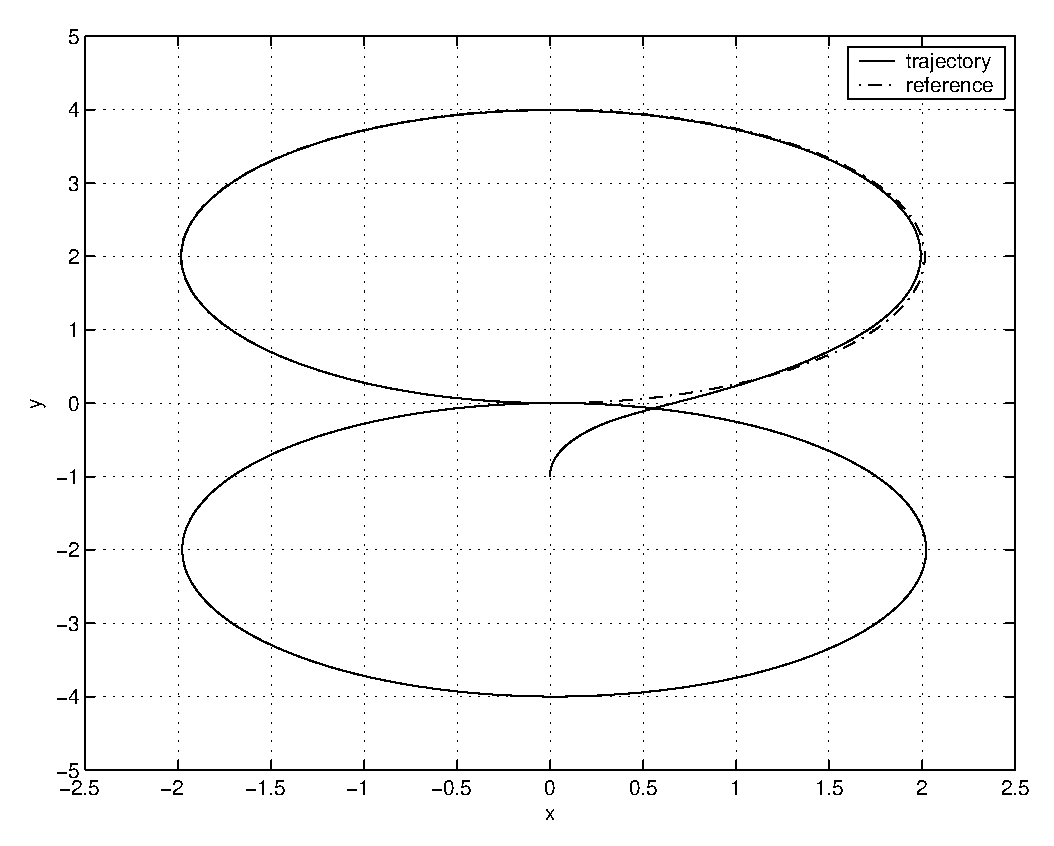
\includegraphics[width=.99\linewidth]{Figures/traj8.eps}
	\caption{Trajectory covered by the WMR, in the $XY$ plane.}
	\label{fig:traj8}
\end{figure}

Fig. \ref{fig:errors} shows the errors of the states converging to zero. The most interesting one is Fig. \ref{fig:controls}. It can be clearly seen that the control inputs obey the limits imposed by the constraints. As the state errors converge to zero (Fig. \ref{fig:errors}), one could say that the value of the cost function must converges to zero too. This fact can be observed in Fig. \ref{fig:cost}.
\begin{figure}
	\centering
	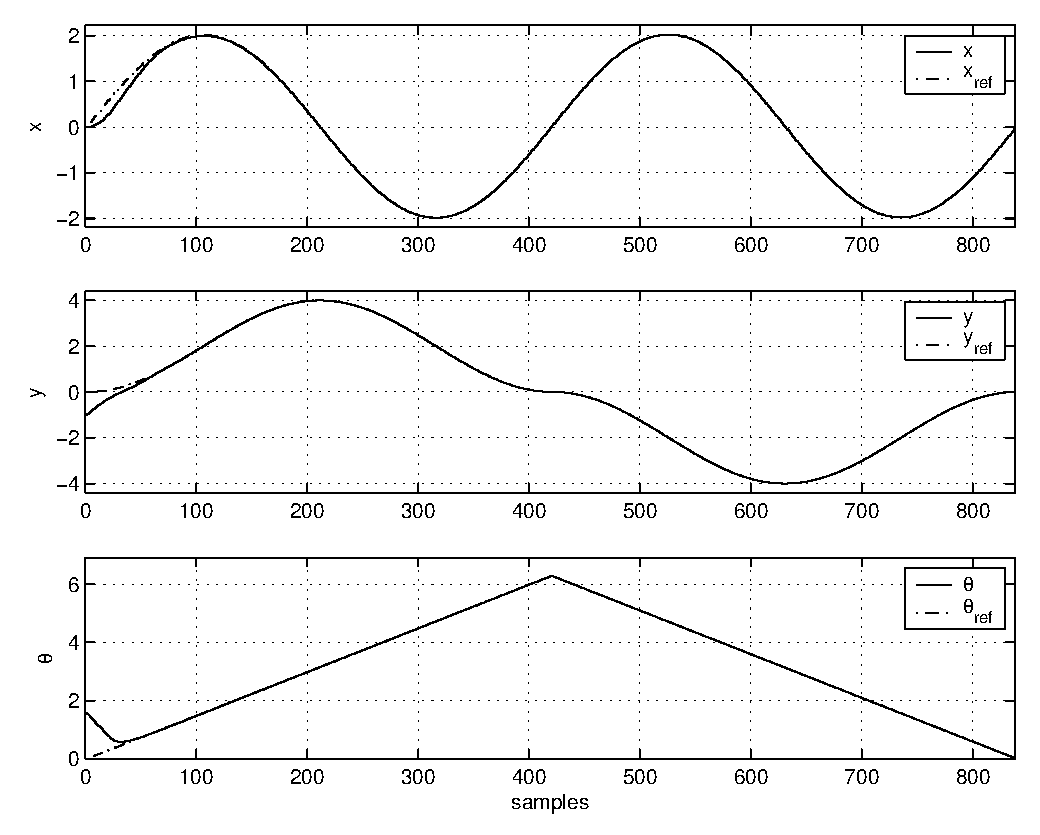
\includegraphics[width=.99\linewidth]{Figures/states.eps}
	\caption{States $x$, $y$ and $\theta$ of the WMR.}
	\label{fig:states}
\end{figure}
\begin{figure}
	\centering
	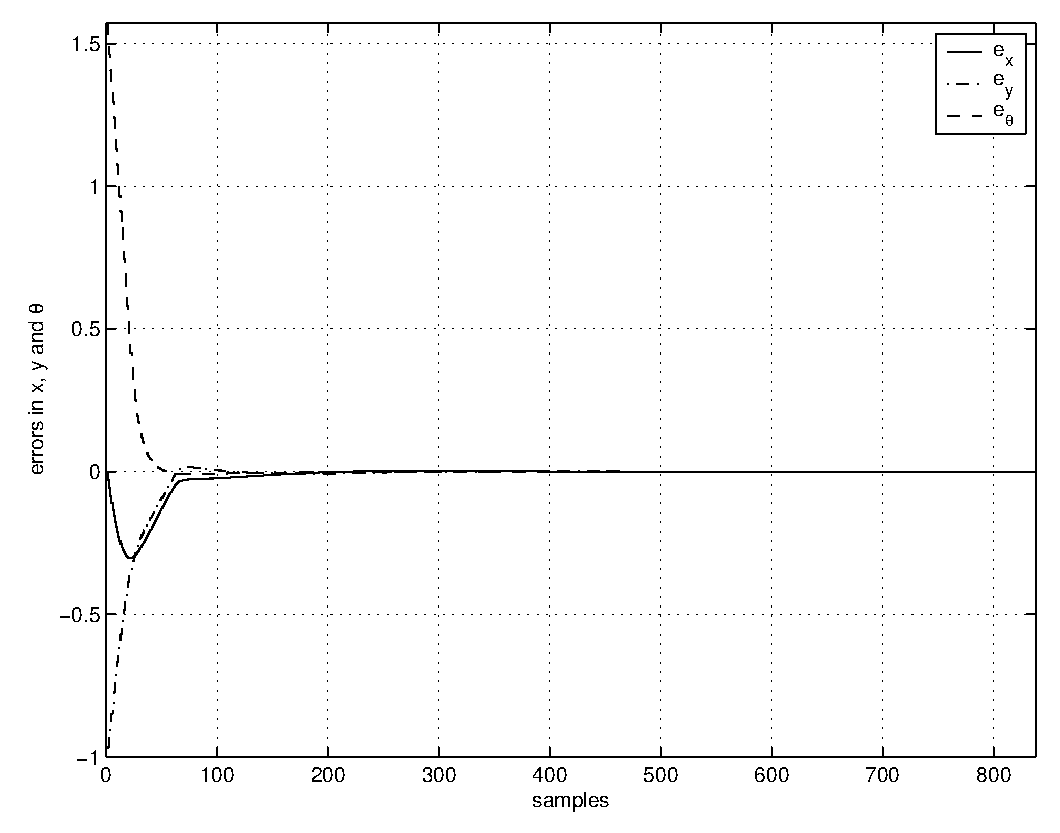
\includegraphics[width=.99\linewidth]{Figures/errors.eps}
	\caption{Errors between states and references.}
	\label{fig:errors}
\end{figure}
\begin{figure}
	\centering
	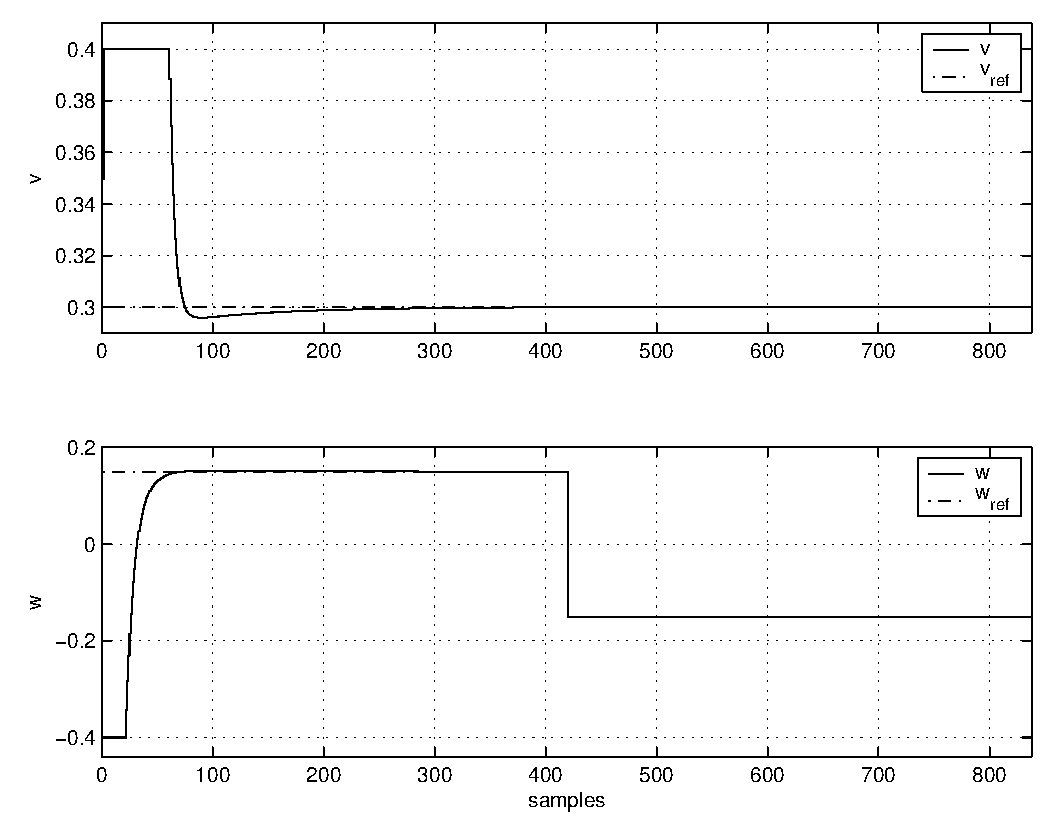
\includegraphics[width=.99\linewidth]{Figures/controls.eps}
	\caption{Controls bounded by the constraints (dotted lines for unconstrained case).}
	\label{fig:controls}
\end{figure}
\begin{figure}
	\centering
	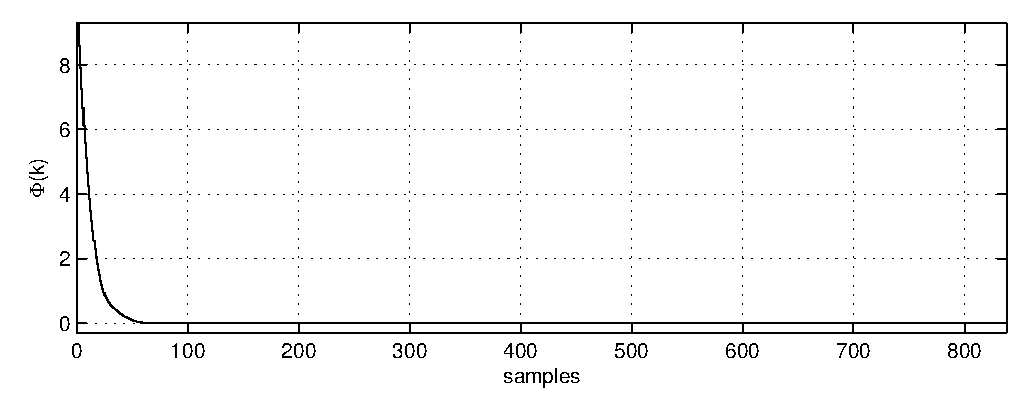
\includegraphics[width=.99\linewidth]{Figures/cost.eps}
	\caption{Value of the cost function $\Phi(k)$.}
	\label{fig:cost}
\end{figure}


\section{Conclusion}\label{sec:conclusions}
This paper has presented the application of MPC to a nonholonomic WMR, represented by means of a kinematic model. It was shown the solution of the optimization problem through a standard QP method. Constraints were imposed on the control variables, which obeyed it perfectly. Such research will obviously continue, and the authors' main objective is real-time simulations of nonlinear model predictive control (NMPC) applied to WMR's.


\subsection*{Acknowledgments}
The authors gratefully acknowledge the financial support from CAPES.

\nocite{*}
\bibliographystyle{IEEEtran}
\bibliography{IEEEabrv,mechrob04_bib}

\end{document}


